\chapter{Renormierung, Natürlichkeit und das Hierarchieproblem}

\lectureoverview{Die zentralen Ideen dieses Kurses gingen aus Fragen zur Renormierung im Standardmodell hervor. Deshalb beginnen wir mit der physikalischen Bedeutung der Renormierung: Freiheitsgrade, die für die jeweilige Fragestellung zu klein und zu schnell sind, werden eliminiert; ihre Auswirkungen werden anschließend in einer effektiven Beschreibung festgehalten. Ein Molekül liefert das Grundmodell. Die Dimensionsanalyse überträgt dieselbe Argumentation dann auf die skalare Quantenfeldtheorie. Dort macht sie die quadratische Empfindlichkeit einer skalaren Masse, das Hierarchieproblem des Higgs-Feldes, den Schutz von Fermionen und Eichbosonen sowie das noch gravierendere Problem der Vakuumenergie sichtbar.}

\section{Physik auf der Skala der jeweiligen Fragestellung}

Die meisten Ideen, die wir in diesem Quartal entwickeln werden, gingen aus Fragen zur Renormierung---manchmal Rätseln, manchmal nützlichen Beobachtungen---im Standardmodell hervor. Die Renormierung verbindet zwei Denkweisen. Bei der ersten entfernt man aus einer Beschreibung Strukturen auf so kurzen Abständen, dass sie für die jeweilige Fragestellung unerheblich sind. Die zweite ist die Dimensionsanalyse, die häufig schon die Antwort für kurze Abstände liefert, bevor irgendein schwieriges Integral ausgewertet wird.

Diese Reduktion von Details findet in der gesamten Physik statt. Um einen Atomkern zu verstehen, können wir bei den Quarks und der Quantenchromodynamik beginnen. Nachdem wir die Massen und Spins von Proton und Neutron sowie ihre effektiven Kernkräfte berechnet haben, können wir ihre Quark-Unterstruktur für viele Zwecke außer Acht lassen. Die Bewegung im Kern ist so langsam, dass eine nichtrelativistische Quantenmechanik von Protonen und Neutronen oft die nützlichere Beschreibung ist.

Auf der nächsten Ebene benötigt die Atomphysik gewöhnlich keine Kenntnis vom inneren Aufbau eines Atomkerns. Die Kernphysik sagt uns, welche Kerne und Isotope existieren, und liefert Eigenschaften wie Masse und elektrische Ladung. Dann beginnen wir mit einem neuen Satz effektiver elementarer Objekte: Kernen und Elektronen. Quarks, Protonen und Neutronen existieren weiterhin; ihre Auswirkungen sind in den Parametern zusammengefasst, die den Kernen zugeordnet sind.

Wie viel beibehalten wird, hängt von der nächsten Fragestellung ab. Für eine atomphysikalische Berechnung kann die Kernmasse nötig sein, weil sie in die reduzierte Masse eingeht; die Ladung wird auf jeden Fall benötigt, weil sie das Coulomb-Feld bestimmt. Üblicherweise muss man nicht wissen, welches Quark welchen Anteil des Kernimpulses trägt. Es gibt etwa neunzig Elementarladungen und, wenn man Isotope mitzählt, noch mehr Kernarten. Dieser Katalog kann als Eingabe dienen. Elektronen lassen sich dagegen noch nicht eliminieren: Ihre Bewegung ist genau das, was die Atomstruktur ausmacht.

Nachdem wir das Atomproblem gelöst haben, können wir Atome ebenso als Bausteine von Molekülen betrachten. Susskinds scherzhafte Aufzählung von Keksatomen, Kaffeeatomen, Schokoladenatomen und Ketchupatomen macht einen ernsthaften Punkt deutlich: Auf jeder Ebene beginnt eine neue Beschreibung. Sind die Eigenschaften und Kräfte der Moleküle bekannt, lassen sie sich zu größeren, tinkertoyartigen Gebilden zusammenfügen, ohne bei jedem Schritt das Elektronenproblem erneut aufzurollen.

Jeder solche Übergang ist eine Grobkörnung. Die neue Beschreibung mag absolut gesehen weniger exakt sein, ist aber auf der vorgesehenen Skala viel nützlicher. In der Quantenfeldtheorie lässt sich diese Frage nicht umgehen, denn ein Feld besitzt Moden jeder Wellenlänge, auch beliebig kurze. Deshalb summieren wir die Auswirkungen von Wellenlängen, die zu kurz sind, um aufgelöst zu werden, und ersetzen sie durch neue effektive Parameter. Das ist zusammen mit der Dimensionsanalyse der physikalische Gehalt der Renormierung.

\section{Ein Molekül als Grundmodell}

Betrachten wir zwei Atome und suchen eine einfache Beschreibung ihrer Relativbewegung. Jedes Atom besteht aus einem schweren Kern und einer Elektronenwolke. Schon ein Proton ist ungefähr zweitausendmal schwerer als ein Elektron; bei schwereren Kernen wird der Skalenunterschied noch größer. Ein anschauliches Bild ist ein Paar Bowlingkugeln, umgeben von schnell umherfliegenden Fliegen: Die Kerne reagieren langsam, während sich der elektronische Zustand rasch neu anordnet.

Die Kernpositionen und -impulse seien \(R_a\) und \(P_a\), bei gleicher Masse \(M\); die Elektronenkoordinaten und -impulse seien \(r_i\) und \(q_i\), bei Masse \(m_e\). Unter Weglassung üblicher Faktoren wie \(4\pi\epsilon_0\) hat der Hamiltonoperator schematisch die Form \begin{align}
H={}&
\frac{P_1^2}{2M}+\frac{P_2^2}{2M}
+\frac{e^2}{R_{12}}
+\sum_i\frac{q_i^2}{2m_e}
+\frac12\sum_{i\ne j}\frac{e^2}{r_{ij}}
\nonumber\\
&-\sum_i\left(
\frac{e^2}{|R_1-r_i|}
+\frac{e^2}{|R_2-r_i|}
\right).
\label{eq:molecular-hamiltonian}
\end{align}In der ersten Zeile stehen die kinetischen Energien der Kerne, ihre gegenseitige Coulomb-Abstoßung und die kinetische Energie der Elektronen. Die zweite Zeile umfasst die Elektron-Elektron-Abstoßung und die Elektron-Kern-Anziehung. Für Kerne mit beliebigen Ladungen werden die entsprechenden Faktoren \(Z_a\) wieder eingesetzt; in der Vorlesung bleiben die Ladungen schematisch, denn entscheidend ist die Trennung der Zeitskalen.

Es gibt zwei charakteristische Bewegungen. Die Kerne sind schwer und langsam; die Elektronen sind leicht und schnell genug, um wie ein verschwommener Fleck zu wirken. In erster Näherung fixieren wir die Kernpositionen und fassen alle von den Elektronen abhängigen Terme in einem elektronischen Hamiltonoperator zusammen, \begin{equation}
H_{\mathrm{el}}(R_1,R_2).
\end{equation}Für jede feste Kernkonfiguration lösen wir \begin{equation}
H_{\mathrm{el}}(R_1,R_2)
\psi_0(r_1,\ldots,r_N;R_1,R_2)
=
E_{\mathrm{el}}(R_1,R_2)\psi_0.
\label{eq:electronic-ground-state}
\end{equation}Wir behalten den niedrigsten elektronischen Eigenwert bei. Die Elektronen wurden nicht ignoriert; ihre gesamte schnelle Bewegung ist in der Funktion \(E_{\mathrm{el}}(R_1,R_2)\) zusammengefasst.

Die Argumentation ist adiabatisch. Während einer schnellen elektronischen Anpassung haben sich die Kerne so wenig bewegt, dass ihre Koordinaten als Parameter behandelt werden können. Nachdem das elektronische Eigenwertproblem gelöst ist, lassen wir dieselben Koordinaten wieder variieren. Bei jeder langsam veränderlichen Konfiguration folgt die Elektronenwolke ihrem momentanen Grundzustand. Eine genauere Behandlung könnte angeregte elektronische Flächen und Übergänge zwischen ihnen berücksichtigen, doch schon die führende Fläche veranschaulicht die Idee der Renormierung.

\begin{figure}[htbp]\centering
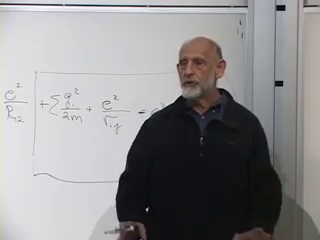
\includegraphics[width=0.72\textwidth]{lecture_01_figure_02.png}\caption{Der molekulare Hamiltonoperator bleibt sichtbar, während das elektronische Grundzustandsproblem eingeführt wird. Die getippte Fassung in Gl.~\eqref{eq:molecular-hamiltonian}hält die Terme fest, die in diesem Bild verdeckt sind.}\lectureframe{00:16:19}\end{figure}

\begin{classroomqa}\audiencequestion{Werden die Kernimpulse einfach auf null gesetzt?\lecturetimestamp{00:15:39}}\lecturerresponse{Nur vorübergehend. In der führenden Näherung behandeln wir die Kerne so, als wären sie festgenagelt, weil sie sich viel langsamer bewegen als die Elektronen. Ihre Impulse werden wieder berücksichtigt, wenn wir das effektive Kernproblem lösen. Diese Näherung verletzt also nicht die Unschärferelation.}\end{classroomqa}

Die Energie des elektronischen Grundzustands trägt nun zum Potenzial bei, das die Kerne erfahren: \begin{equation}
V_{\mathrm{eff}}(R_1,R_2)
=\frac{e^2}{R_{12}}+E_{\mathrm{el}}(R_1,R_2).
\label{eq:molecular-effective-potential}
\end{equation}Rotations- und Translationsinvarianz reduzieren es für zwei isolierte Atome auf eine Funktion ihres Abstands \(R_{12}\). Bei sehr kleinen Abständen dominiert die Coulomb-Abstoßung der Kerne. Bei sehr großen Abständen ist die Wechselwirkung schwach. Dazwischen kann die Elektronenwolke einen anziehenden Bereich und ein Minimum erzeugen. Die Kernwellenfunktion liegt dann in der Nähe dieses Minimums und beschreibt ein gebundenes Molekül.

Beachten Sie die Reihenfolge der Schritte. Wir haben keine empirische Anziehungskraft angenommen und die Elektronen verworfen. Zuerst haben wir ihr Quantenproblem im festen Kernhintergrund gelöst. Erst danach haben wir ihre expliziten Koordinaten aus der Beschreibung entfernt und den daraus hervorgehenden Eigenwert beibehalten. Die Physik auf kurzen Abständen bleibt in Form, Tiefe und Krümmung von \(V_{\mathrm{eff}}\) erhalten. Die Lage seines Minimums legt den Gleichgewichtsabstand fest, seine Krümmung bestimmt kleine Schwingungen und sein asymptotisches Verhalten entscheidet darüber, ob ein gebundener Zustand existiert. Eine effektive Funktion überträgt all diese Informationen der Elektronen in das langsamere Problem.

So ist aus einem komplizierten Hamiltonoperator für viele Elektronen ein Hamiltonoperator für zwei Kerne mit einem neuen Potenzial geworden. Wir haben die schnellen Freiheitsgrade eliminiert, aber ihre gesamte Wirkung bei niedrigen Energien beibehalten. Das Potenzial wurde renormiert. Diese vertraute Born--Oppenheimer-Argumentation wird üblicherweise nicht unter diesem Namen eingeführt, enthält aber genau die Idee, die wir benötigen: \begin{equation}
\begin{gathered}
\text{fast microscopic dynamics}\\
\Downarrow\\
\text{effective parameters for slow dynamics}
\end{gathered}
\end{equation}

\section{Natürliche Einheiten und die Dimension eines Feldes}

In der Quantenfeldtheorie lassen sich die zu eliminierenden Moden gleichbedeutend als Moden auf kurzen Abständen, mit kurzen Wellenlängen, hohen Frequenzen oder hohen Energien beschreiben. Bevor wir Diagramme zeichnen, klären wir die Dimensionszählung.

In der gewöhnlichen Mechanik verwendet man unabhängige Einheiten für Länge, Zeit und Masse. In der Teilchenphysik setzen wir \begin{equation}
\hbar=c=1.
\end{equation}. Damit sind Energie und Masse über \(E=mc^2\) äquivalent, Länge und Zeit wegen \(c=1\) ebenfalls, und \(\hbar=1\) macht den Impuls zum Kehrwert der Länge. Es bleibt nur eine Dimension: \begin{equation}
[M]=[E]=[p]=L^{-1},
\qquad
[x]=[t]=L.
\label{eq:natural-units}
\end{equation}

Dadurch verschwinden die Dimensionen nicht. Vielmehr wählt man Umrechnungsfaktoren so, dass sich eine Zeit als Länge und eine Masse als Kehrwert einer Länge angeben lässt. Sobald eine Einheit festgelegt ist, ergeben sich alle anderen daraus. Deshalb kann man einen Cutoff entweder als kurzen Abstand \(\delta\) oder als hohe Energie \(\Lambda=1/\delta\) beschreiben: In beiden Fällen handelt es sich um dieselbe Skala, ausgedrückt in zwei Sprachen.

Betrachten wir ein reelles Skalarfeld \(\phi\) mit schematisch normierter Lagrangedichte \begin{equation}
\mathcal L=(\partial_\mu\phi)(\partial^\mu\phi)-V(\phi),
\qquad
S=\int d^4x\,\mathcal L.
\label{eq:scalar-action}
\end{equation}

\begin{figure}[htbp]\centering
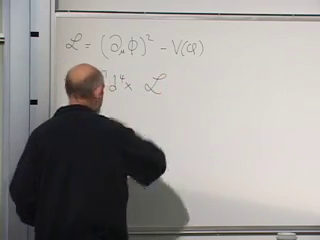
\includegraphics[width=0.78\textwidth]{lecture_01_figure_03.png}\caption{Die lokale skalare Lagrangedichte und ihr Raumzeitintegral, die Wirkung.}\lectureframe{00:26:08}\end{figure}

Die Lagrangedichte ist lokal: Sie beschreibt einen einzelnen Raumzeitpunkt. Die klassischen Feldgleichungen erhält man, indem man die Wirkung stationär macht. In der Quantentheorie tritt dieselbe Wirkung in der Phase des Pfadintegrals \(\exp(iS)\) auf. Bei beiden Betrachtungsweisen ist die Dimension von \(S\) entscheidend. Setzen wir \(\hbar\) wieder ein, lautet die Phase \(\exp(iS/\hbar)\); nach der Festlegung \(\hbar=1\) muss \(S\) selbst dimensionslos sein.

\begin{classroomqa}\audiencequestion{Hat die Wirkung Einheiten von \(\hbar\)?\lecturetimestamp{00:26:13}}\lecturerresponse{Ja. Da \(\hbar\) gleich eins gesetzt wurde, ist die Wirkung in diesen Einheiten dimensionslos. Das vierdimensionale Maß hat die Dimension \(L^4\), daher muss die Lagrangedichte die Dimension \(L^{-4}\) haben.}\end{classroomqa}

Der kinetische Term legt nun die Dimension des Feldes fest: \begin{align}
[S]&=1, & [\mathcal L]&=L^{-4},\\
[\partial_\mu]&=L^{-1}, &
[(\partial\phi)^2]&=L^{-2}[\phi]^2=L^{-4},\nonumber\\
&& [\phi]&=L^{-1}.
\label{eq:scalar-dimension}
\end{align}Diese kurze Rechnung wird die Größe sämtlicher folgenden Diagramme im ultravioletten Bereich bestimmen.

Entwickeln wir das Potenzial in eine Reihe: \begin{equation}
V(\phi)=\frac{m^2}{2}\phi^2+g\phi^3+\lambda\phi^4+\cdots.
\label{eq:scalar-potential}
\end{equation}Jeder Term muss die Dimension \(L^{-4}\) haben. Da \([\phi^n]=L^{-n}\)\begin{equation}
[m^2]=L^{-2},
\qquad
[g]=L^{-1},
\qquad
[\lambda]=1.
\label{eq:coupling-dimensions}
\end{equation}Die quartische Kopplung ist dimensionslos. Solche Kopplungen sind für die Renormierung besonders wichtig, weil sich ihre Skalenabhängigkeit nicht direkt aus einer einfachen Potenz der Länge ablesen lässt.

\begin{classroomqa}\audiencequestion{Hat \(g\) die Dimension einer Masse?\lecturetimestamp{00:29:52}}\lecturerresponse{Ja. Der Faktor \(\phi^3\) hat die Dimension \(L^{-3}\), während die Potenzialdichte die Dimension \(L^{-4}\) haben muss. Folglich gilt \([g]=L^{-1}\), also hat die Größe in natürlichen Einheiten die Dimension einer Masse.}\end{classroomqa}

\section{Vertizes und der Propagator auf kurzen Abständen}

Die Feynman-Regeln setzen sich aus Vertizes und Propagatoren zusammen. Der Term \(g\phi^3\) liefert einen Vertex mit drei Linien und einem Faktor proportional zu \(g\); der Term \(\lambda\phi^4\) liefert einen Vertex mit vier Linien und einem Faktor proportional zu \(\lambda\). Der quadratische Term ergibt eine lokale Zweipunkt-Einfügung. Man kann sie als ein Teilchen darstellen, das eintritt, absorbiert und wieder emittiert wird; ihr Koeffizient ist proportional zu \(m^2/2\). Numerische Normierungen, Vorzeichen, Faktoren von \(i\) und Symmetriefaktoren werden bewusst weggelassen, denn in der Vorlesung geht es um die Skalenabhängigkeit und nicht um die Berechnung eines Wirkungsquerschnitts.

Diese Zeichnungen lassen sich unmittelbar physikalisch deuten. Ein Dreipunktvertex kann zwei Quanten absorbieren und eines emittieren oder eine beliebige kreuzungsbezogene Zuordnung seiner drei Linien darstellen. Ein Vierpunktvertex kann den Ein- und Austritt von je zwei Teilchen beschreiben. Das quadratische Kreuz ist ebenfalls ein zulässiger Zweilinienvertex, obwohl man es normalerweise in den freien Propagator aufnimmt. Wir zeigen es, weil sich jeder nicht aufgelöste Zweipunktprozess gleich daran erkennen lässt.

Ein Propagator verbindet zwei Raumzeitpunkte. Seine Linie behauptet nicht, dass sich ein Quantenobjekt auf einer geraden klassischen Bahn bewegt hat. Sie steht für die Amplitude, am Punkt \(x\) eine Feldanregung zu erzeugen und sie am Punkt \(y\) zu entfernen oder nachzuweisen: \begin{equation}
\Delta(x-y)=\langle0|\phi(y)\phi(x)|0\rangle.
\label{eq:position-propagator}
\end{equation}Lesen Sie den Ausdruck von rechts nach links. Die Wirkung von \(\phi(x)\) auf das Vakuum erzeugt bei \(x\) einen Einteilchenanteil. Die Wirkung von \(\phi(y)\) auf den Bra-Vektor entfernt den Anteil bei \(y\). Ihr Vakuummatrixelement ist die Überlappungsamplitude dafür, dass am ersten Punkt ein Teilchen erzeugt und am zweiten nachgewiesen wird. Die Symbole \(x\) und \(y\) bezeichnen vollständige Vierervektoren, nicht bloß zwei kartesische Koordinaten.

Zustände tragen keine physikalische Dimension, während jedes Feld den Faktor \(L^{-1}\) beiträgt. Daher gilt \begin{equation}
[\Delta]=L^{-2}.
\end{equation}Für ein masseloses Feld gibt es keine intrinsische Längenskala. Deshalb erzwingt die Dimensionsanalyse das Verhalten auf kurzen Abständen \begin{equation}
\Delta(x-y)\sim\frac{1}{(x-y)^2}.
\label{eq:massless-propagator}
\end{equation}Der Nenner ist der lorentzinvariante quadrierte Abstand, ergänzt um die übliche Vorschrift für seine Singularitäten.\editorialnote{Für die Potenzzählung ist eine Wick-Rotation zum euklidischen Abstand praktisch; dort ist der Betrag eindeutig proportional zu \(1/|x-y|^2\). Die für die folgende Rechnung verwendeten ultravioletten Potenzen ändern sich dadurch nicht.}

Wenn \(y\) gegen \(x\) geht, divergiert der Propagator. Diese Singularität bei Ausbreitung über einen verschwindenden Abstand ist der Ursprung, aus dem die ultravioletten Divergenzen komplizierterer Diagramme hervorgehen.

\section{Renormierung einer skalaren Masse}

Für ein Skalarfeld ist \(m^2\) der dynamische Parameter, wie schon die relativistische Dispersionsrelation nahelegt: \begin{equation}
E=\sqrt{\mathbf p^2+m^2}.
\end{equation}Sei \(\delta\) der kleinste Abstand, den unsere effektive Beschreibung auflöst. Prozesse, deren Vertizes weniger als \(\delta\) voneinander entfernt sind, unterscheiden wir nicht. Jeder derartige, nicht aufgelöste Prozess mit einem einlaufenden und einem auslaufenden Skalar hat dieselbe beobachtbare Zweipunktstruktur wie eine Masseneinfügung und muss daher zur effektiven Masse beitragen.

Man kann sich einen Beschleuniger als Mikroskop vorstellen. Beträgt seine höchste Auflösung \(\delta\), lässt sich eine Absorption an einem Punkt mit anschließender Emission in einem viel kleineren Abstand als \(\delta\) nicht von einem tatsächlich lokalen Ereignis unterscheiden. Wir verwischen den Vertex gezielt über diese Skala. Die Renormierung ist die Vorschrift, alle solchen Alternativen unterhalb der Auflösungsgrenze in den Koeffizienten des entsprechenden lokalen Operators aufzunehmen.

\subsection{Die erste quartische Korrektur}

Beginnen wir mit einem einzelnen Vertex der Wechselwirkung \(\phi^4\). Zwei Beine gehören zum äußeren Teilchen; die beiden anderen schließen sich zu einer kurzen Schleife, die nahe demselben Punkt emittiert und wieder absorbiert wird. Verschmieren wir den Propagator am zusammenfallenden Punkt über die Cutoff-Länge, erhalten wir \begin{equation}
\Delta(0)\ \longrightarrow\ \Delta(\delta)\sim\frac{1}{\delta^2},
\end{equation}und damit \begin{equation}
\delta m^2_{(1)}\sim\frac{\lambda}{\delta^2}.
\label{eq:one-loop-scalar-mass}
\end{equation}Bezeichne \(m_0^2\) den Eingabe- oder nackten Parameter, so hat der Zweipunktkoeffizient bei niedriger Auflösung schematisch die Form \begin{equation}
\frac{m_{\mathrm{eff}}^2}{2}
\sim
\frac{m_0^2}{2}
+c_1\frac{\lambda}{\delta^2},
\label{eq:first-renormalized-mass}
\end{equation}Dabei umfasst \(c_1\) die weggelassenen numerischen und konventionsabhängigen Faktoren. Die in Experimenten gemessene Labormasse, bei denen Abstände unterhalb von \(\delta\) nicht aufgelöst werden, ist diese renormierte Größe und nicht \(m_0\) für sich genommen.

Das beobachtete Zweipunktereignis kann also auf zwei ununterscheidbare Arten zustande kommen. Der ursprüngliche quadratische Vertex kann das Teilchen absorbieren und wieder emittieren, oder die quartische Wechselwirkung kann dies tun, indem sie kurzzeitig ein virtuelles Skalarteilchen emittiert und wieder absorbiert. In der Quantenmechanik werden die Amplituden addiert. Sobald die Schleife unterhalb der Auflösungsgrenze liegt, verschwindet ihr eigener Ablauf aus der effektiven Beschreibung, ihr Beitrag zum gemessenen Koeffizienten bleibt jedoch erhalten.

\subsection{Die nächste quartische Korrektur}

Verbinden wir nun zwei quartische Vertizes so, dass bei \(x\) ein äußeres Teilchen einläuft, bei \(x+\Delta\) eines ausläuft und drei interne Propagatoren die Vertizes verbinden. Es treten zwei Potenzen von \(\lambda\) auf, während die Propagatoren den Faktor \(\Delta^{-6}\) liefern. Quantenamplituden müssen über alle nicht aufgelösten Orte summiert werden, an denen das auslaufende Teilchen entstehen kann. Daher integrieren wir über den relativen Vierervektor: \begin{equation}
\delta m^2_{(2)}
\sim
\lambda^2
\int_{|\Delta|\gtrsim\delta}
d^4\Delta\,\frac{1}{|\Delta|^6}.
\label{eq:two-loop-power-count}
\end{equation}

\begin{classroomqa}\audiencequestion{Bedeutet die kleine Markierung am Vertex, dass dort nur drei Teilchen zusammentreffen?\lecturetimestamp{00:46:35}}\lecturerresponse{Nein. Wir verwenden weiterhin die quartische Wechselwirkung. An jedem Vertex treffen vier Linien zusammen; in diesem Zweipunktdiagramm ist eine davon außen, während drei zwischen den beiden Vertizes verlaufen. Am zweiten Vertex treffen ebenfalls vier Linien zusammen.}\end{classroomqa}

Das Maß liefert vier Längenpotenzen, die drei Propagatoren dagegen minus sechs. Da der ultraviolette Cutoff die einzige Skala der Abschätzung ist, gilt \begin{equation}
\int_{|\Delta|\gtrsim\delta}
\frac{d^4\Delta}{|\Delta|^6}
\sim\frac{1}{\delta^2},
\qquad
\delta m^2_{(2)}
\sim\frac{\lambda^2}{\delta^2}.
\label{eq:two-loop-scalar-mass}
\end{equation}Hier ist \(\Delta^\mu\) eine vierkomponentige Integrationsvariable; integriert wird über die Zeit- und die drei Raumkomponenten. Das kleine \(\delta\) ist der festgelegte Cutoff. In der Vorlesung wird zunächst derselbe Name für beide verwendet, die Notation wird später berichtigt.

Dasselbe Ergebnis zeigt sich, wenn man das vierdimensionale Maß in Radialkoordinaten schreibt. Bis auf einen Winkelanteil gilt \begin{equation}
\int_{\delta}\frac{d^4\Delta}{|\Delta|^6}
\sim
\int_{\delta}\frac{R^3\,dR}{R^6}
=\int_{\delta}\frac{dR}{R^3}
\sim\frac{1}{\delta^2}.
\end{equation}Deshalb ist die obere Grenze bei großen Abständen für die ultraviolette Abschätzung unerheblich: Das Integral wird von seiner unteren Grenze dominiert.

Bei höheren Diagrammen wiederholt sich dieses Muster. Ein Diagramm mit mehr quartischen Vertizes bringt eine höhere Potenz von \(\lambda\) mit sich, doch die Dimensionsanalyse lässt weiterhin einen quadratisch divergenten Beitrag zur Masse zu: \begin{equation}
\begin{aligned}
m_{\mathrm{eff}}^2
={}&m_0^2
+\frac{1}{\delta^2}
\left(c_1\lambda+c_2\lambda^2+c_3\lambda^3+\cdots\right)\\
&+\text{weaker terms}.
\end{aligned}
\label{eq:scalar-mass-series}
\end{equation}

\subsection{Die kubische Wechselwirkung und ein Logarithmus}

Zwei kubische Vertizes enthalten zwei Propagatoren zwischen nahe beieinanderliegenden Punkten. Ihr Beitrag skaliert wie \begin{equation}
\delta m_g^2
\sim
g^2\int_{|\Delta|\gtrsim\delta}
\frac{d^4\Delta}{|\Delta|^4}.
\label{eq:cubic-loop}
\end{equation}Nun tragen Maß und Nenner dieselben Potenzen. Die verbleibende Abhängigkeit ist daher logarithmisch statt einer Potenz: \begin{equation}
\delta m_g^2
\sim
c_g g^2\log\!\left(\frac{1}{\mu\delta}\right).
\label{eq:cubic-log}
\end{equation}Die Referenzskala \(\mu\) macht den Logarithmus dimensionslos. Dies ist die vollständig dimensionierte Fassung des schematischen Ausdrucks \(g^2\log\delta\) aus der Vorlesung. Ein Logarithmus ändert sich viel langsamer als jede inverse Potenz, daher dominiert \(1/\delta^2\), wenn der Cutoff klein wird.

Auch die radiale Form macht den Unterschied deutlich: \begin{equation}
\int_{\delta}^{R_{\mathrm{IR}}}
\frac{d^4\Delta}{|\Delta|^4}
\sim
\int_{\delta}^{R_{\mathrm{IR}}}\frac{R^3\,dR}{R^4}
=\log\!\left(\frac{R_{\mathrm{IR}}}{\delta}\right).
\end{equation}Gleiche Potenzen im Maß und im Nenner ergeben einen Logarithmus. Höhere Potenzen im Nenner ergeben eine inverse Potenz des Cutoffs. In der Vorlesung sollen wir keine Winkelanteile ausrechnen, sondern lernen, das ultraviolette Ergebnis auf Anhieb zu erkennen.

\begin{classroomqa}\audiencequestion{Zu welcher Basis gehört der Logarithmus?\lecturetimestamp{00:57:42}}\lecturerresponse{Verwenden Sie den natürlichen Logarithmus. Ein Wechsel der Basis ändert lediglich einen numerischen Faktor, der in den Koeffizienten aufgenommen wird. Die Faktoren von \(2\) und \(\pi\) sowie die Symmetriefaktoren sind hier nicht berechnet worden.}\end{classroomqa}

\begin{classroomqa}\audiencequestion{Wie kann man den Logarithmus einer Länge bilden, und woher stammen die Einheiten der Massenkorrektur?\lecturetimestamp{00:58:32}}\lecturerresponse{Ein Logarithmus vergleicht immer zwei Skalen; genau genommen ist es der Logarithmus eines dimensionslosen Verhältnisses wie \(1/(\mu\delta)\). Die Kopplung \(g\) hat die Dimension einer Masse, sodass \(g^2\) bereits genau die für die Korrektur erforderliche Dimension einer quadrierten Masse besitzt.}\end{classroomqa}

\begin{classroomqa}\audiencequestion{Liefert ein Feynman-Diagramm eine Amplitude. Ist ihr Betragsquadrat eine Wahrscheinlichkeit?\lecturetimestamp{00:59:41}}\lecturerresponse{Ja, wenn die Amplitude mit den erforderlichen Zustands- und Phasenraumfaktoren in eine physikalische Übergangsrechnung eingeht. Hier spielt sie eine unmittelbar andere Rolle: Eine nicht aufgelöste Zweipunktamplitude hat dieselbe lokale Form wie der Massenterm und verschiebt deshalb den effektiven Massenparameter.}\end{classroomqa}

\section{Jeder Parameter wird effektiv}

Die unendliche Familie von Massendiagrammen verschwindet nicht bloß deshalb, weil \(\lambda\) klein ist. Die Störungstheorie ordnet sie nach Potenzen der Kopplung, sodass aufeinanderfolgende Terme kleiner werden können; dennoch bleiben es unendlich viele. Dieselbe Elimination der Physik auf kurzen Abständen renormiert auch die Wechselwirkungen selbst.

\begin{classroomqa}\audiencequestion{Gibt es nicht selbst bei der Massenrenormierung unendlich viele Diagramme?\lecturetimestamp{01:00:35}}\lecturerresponse{Doch. Wenn \(\lambda\) hinreichend klein ist, kann die Störungsreihe nützlich sein, weil aufeinanderfolgende höhere Potenzen unterdrückt sind. Trotzdem wird der renormierte Parameter durch die gesamte Reihe definiert und nicht nur durch die erste Zeichnung.}\end{classroomqa}

Operativ betrachtet entspricht eine lokale Wechselwirkung \(\lambda\phi^4\) einer Amplitude mit zwei einlaufenden und zwei auslaufenden Teilchen. Findet ein komplizierterer Vierpunktprozess vollständig in einem nicht aufgelösten Bereich statt, ist er bei niedriger Auflösung vom ursprünglichen lokalen Vertex nicht zu unterscheiden. Solche Diagramme werden daher in einer effektiven Kopplung \(\lambda\) zusammengefasst. Ihre führende Skalenabhängigkeit ist in einer vierdimensionalen \(\phi^4\)-Theorie typischerweise logarithmisch. Die Vorlesung berechnet diese Betafunktion nicht, sondern führt das Beispiel für eine allgemeine Aussage an: \begin{equation}
\begin{gathered}
\text{parameters measured at low energy}\\
\ne\\
\text{parameters entered at the microscopic cutoff}
\end{gathered}
\end{equation}

Das Vierpunktbeispiel ist wichtig, weil es einem möglichen Missverständnis vorbeugt. Die Renormierung ist keine spezielle Korrektur, die nur auf eine Massendivergenz angewendet wird. Jeder im Lagrange-Ausdruck zulässige Operator kann durch nicht aufgelöste Diagramme mit denselben äußeren Beinen und Symmetrien reproduziert werden. Ein Zweipunktprozess renormiert einen quadratischen Koeffizienten, ein Vierpunktprozess einen quartischen Koeffizienten, und Prozesse vom Vakuum ins Vakuum renormieren den konstanten Term. Die Niederenergie-Lagrangedichte ist das kompakte Verzeichnis, in dem alle diese Prozesse auf kurzen Abständen festgehalten werden.

\begin{classroomqa}\audiencequestion{Da \(\Delta\) die Einheit einer Länge hat, ist sein Logarithmus dann nicht dimensionsmäßig problematisch? Und wurden an der Tafel großes und kleines Delta vertauscht?\lecturetimestamp{01:01:34}}\lecturerresponse{Der Logarithmus bezeichnet tatsächlich das Verhältnis zu einer anderen Skala und ist daher dimensionslos. Ja, die Notation wurde kurzzeitig vertauscht: \(\Delta^\mu\) ist die Integrationsvariable, während \(\delta\) der untere Abstands-Cutoff ist, der im Ergebnis verbleibt.}\end{classroomqa}

Dies ist das Gegenstück des Molekülbeispiels in der Feldtheorie. Wir haben die nicht sichtbaren schnellen Elektronen berechnet und ihr Ergebnis in ein Potenzial aufgenommen. Hier summieren wir die nicht sichtbaren Prozesse auf kurzen Abständen und nehmen ihr Ergebnis in Massen, Kopplungen und jeden anderen zulässigen lokalen Koeffizienten auf. Alles wird verschoben.

\begin{classroomqa}\audiencequestion{Könnten Sie noch einmal erklären, ob die gemessene Größe Skalen einschließt, die das Experiment nicht auflösen kann?\lecturetimestamp{01:05:13}}\lecturerresponse{Ja. Die einzelnen Fluktuationen werden zwar nicht aufgelöst, ihre summierte Wirkung ist jedoch enthalten. Alle Diagramme mit kürzeren Skalen werden im einzelnen effektiven Koeffizienten zusammengefasst, den ein Niederenergieexperiment beispielsweise als physikalische quadrierte Masse misst.}\end{classroomqa}

\begin{classroomqa}\audiencequestion{Muss sich der Eingabeterm \(m_0^2\) dann gegen die anderen Beiträge aufheben?\lecturetimestamp{01:06:00}}\lecturerresponse{Wenn die gemessene skalare Masse viel kleiner ist als die einzelnen ultravioletten Beiträge, ja. Diese erforderliche Aufhebung ist das Problem der Feinabstimmung, dem wir uns nun zuwenden.}\end{classroomqa}

\section{Das Hierarchieproblem des Higgs-Feldes}

Nehmen wir an, der Cutoff entspreche der Planck-Länge. Dann soll die effektive Feldtheorie Fluktuationen von Laborskalen bis hin zu der Skala zusammenfassen, auf der die Quantengravitation eingreifen muss. In Einheiten der Teilchenphysik gilt \begin{equation}
\delta\sim M_{\mathrm{Pl}}^{-1}\sim10^{-19}\,\mathrm{GeV}^{-1},
\qquad
\frac{1}{\delta^2}\sim10^{38}\,\mathrm{GeV}^2.
\label{eq:planck-cutoff}
\end{equation}Ob man dabei die reduzierte oder die nicht reduzierte Planck-Skala verwendet, spielt für den enormen Größenvergleich keine Rolle.

Auch die Längenskalenhierarchie ist erstaunlich. Die Planck-Länge ist etwa neunzehn Größenordnungen kleiner als der Protonenradius und ungefähr sechzehn oder siebzehn Größenordnungen kleiner als die Abstände, die mit den hier besprochenen Beschleunigern direkt untersucht werden. Wenn man dieses Skalenverhältnis quadriert, wird aus der großen Längenhierarchie die erforderliche Aufhebung auf etwa vierunddreißig Dezimalstellen bei einem skalaren Massenquadratparameter.

Für das Higgs-Feld, ein Skalarfeld, liegt die gewünschte elektroschwache Skala bei einigen hundert GeV, nicht bei \(10^{19}\) GeV. Die Terme in Gl.~\eqref{eq:scalar-mass-series} können jedoch natürlicherweise die Größe der Planck-Skala haben. Ihre Vorzeichen wurden nicht berücksichtigt: Einige können positiv und andere negativ sein; auch das nackte Massenquadrat kann jedes der beiden Vorzeichen haben. Damit als Resultat eine Skala der elektroschwachen Wechselwirkung übrig bleibt, müssen sich diese riesigen Beiträge jedoch auf etwa vierunddreißig Dezimalstellen aufheben. Susskind nennt zunächst siebzehn Stellen, korrigiert sich dann aber, weil hier quadrierte Massen verglichen werden. Das quadrierte Verhältnis gibt das Maß dieser Feinabstimmung an.

\begin{classroomqa}
\audiencequestion{Ist \(\lambda\) kleiner oder größer als
1?\lecturetimestamp{01:09:50}}
\lecturerresponse{Man nimmt an, dass sie etwas kleiner als 1 ist. Die Störungstheorie wäre nicht mehr handhabbar, wenn die aufeinanderfolgenden Potenzen anwüchsen; außerdem lässt sich eine reine Skalertheorie bei beliebig großer quartischer Kopplung nicht konsistent extrapolieren. Aber \(\lambda\) ist längst nicht so klein wie \(10^{-38}\); zur Orientierung setzt die Vorlesung einen Wert in der Größenordnung von Prozenten an.}
\end{classroomqa}

\begin{classroomqa}
\audiencequestion{Selbst wenn \(\lambda<1\) gilt, bleiben doch viele Terme wichtig, weil jeder von ihnen den großen Cutoff-Faktor enthält?\lecturetimestamp{01:10:43}}
\lecturerresponse{Ja. Höhere Potenzen unterdrücken die Reihe schließlich, aber bis dahin kann eine große Zahl von Termen beitragen. Diese Terme und der nackte Term müssten sich alle so abstimmen, dass als Ergebnis der außerordentlich kleine physikalische Wert übrig bleibt.}
\end{classroomqa}

Erinnern wir uns daran, warum bekannt ist, dass der Higgs-Massenparameter auf der Skala der schwachen Wechselwirkung liegt. In der Konvention der Vorlesung schreiben wir das Potential mit spontaner Symmetriebrechung als
\begin{equation}
V(\phi)=-\frac{\mu^2}{2}\phi^2+\frac{\lambda}{4}\phi^4.
\label{eq:higgs-potential}
\end{equation}
Der negative quadratische Koeffizient macht den Ursprung instabil, während der positive quartische Term das Potential stabilisiert. Durch Ableiten erhält man
\begin{equation}
\frac{dV}{d\phi}=-\mu^2\phi+\lambda\phi^3
=\phi(-\mu^2+\lambda\phi^2),
\end{equation}
und damit das von null verschiedene Minimum
\begin{equation}
\phi_{\min}^2=f^2=\frac{\mu^2}{\lambda}.
\label{eq:higgs-minimum}
\end{equation}
An der Tafel wird der quartische Term schematisch als \(\lambda\phi^4\) geschrieben, zugleich aber Gl.~\eqref{eq:higgs-minimum} angegeben; setzt man den konventionellen Faktor \(1/4\) ein, stimmen die beiden Zeilen überein, ohne dass sich an der Argumentation etwas ändert.

Das Vorzeichen von \(-\mu^2\) ist wichtig, löst aber das Natürlichkeitsproblem nicht. Die negative Krümmung am Ursprung treibt die spontane Symmetriebrechung an. Durch die Renormierung wird diese Krümmung um große positive und negative Beiträge verschoben. Für das beobachtete gebrochene Vakuum müssen sich diese Beiträge nicht nur zu einem kleinen Wert summieren, sondern zu genau dem kleinen negativen Wert, bei dem das Minimum auf der Skala der schwachen Wechselwirkung liegt.

Die Massen der \(W\)- und \(Z\)-Bosonen legen \(f\) in der groben, in der Vorlesung verwendeten Normierung auf eine Größenordnung von \(200\,\mathrm{GeV}\) fest. Wenn \(\lambda\) weder enorm groß noch außerordentlich klein ist, muss \(\mu\) ungefähr in derselben Größenordnung liegen. Der beobachtete Koeffizient auf der Skala der schwachen Wechselwirkung ist somit der Rest von Beiträgen, die jeweils um Dutzende Größenordnungen größer sein können.

Dies wird als Higgs-Feinabstimmungsproblem, Hierarchieproblem oder Eichhierarchieproblem bezeichnet. Die Hierarchie ist das immense Verhältnis zwischen der gewöhnlichen Skala der schwachen Wechselwirkung und einer möglichen Vereinheitlichungs- oder Planck-Skala. Eine kleine Zahl für sich genommen muss kein Paradoxon sein. Beunruhigend ist hier, dass sich eine kleine Zahl aus großen, scheinbar voneinander unabhängigen Beiträgen zusammensetzt, die sich mit äußerster Präzision aufheben müssen. Das Problem wurde in den späten 1970er Jahren und frühen 1980er Jahren erkannt; die Suche nach einem Mechanismus, der dieser Aufhebung zugrunde liegt, motiviert die Supersymmetrie und mehrere konkurrierende Ideen.

Die unendliche Störungsreihe verschärft das Rätsel, statt es zu beseitigen. Bei einem \(\lambda\) in der Größenordnung von Prozenten werden hinreichend hohe Potenzen klein, aber zuvor können viele Terme auftreten. Es reicht nicht aus, wenn sich eine Schleife zufällig mit der nackten Masse aufhebt. Die effektive Skala der schwachen Wechselwirkung muss stabil bleiben, wenn auch die übrigen kurzreichweitigen Prozesse berücksichtigt werden. Eine strukturelle Beziehung zwischen den Termen wäre eine Erklärung; eine unabhängige, Ziffer für Ziffer abgestimmte Aufhebung ist lediglich eine Feinabstimmung.

\section{Warum sich eine Fermionmasse besser verhält}

Für die anderen Teilchen des Standardmodells sind keine unabhängigen Feinabstimmungen derselben Art erforderlich. Für ein Dirac-Fermion lautet der Massenterm
\begin{equation}
\mathcal L_m=-m\bar\psi\psi
=-m\left(\bar\psi_L\psi_R+\bar\psi_R\psi_L\right).
\label{eq:fermion-mass}
\end{equation}
Er enthält die Masse, nicht deren Quadrat, und koppelt die linke und rechte Chiralität. Eine lokale Masseneinsetzung wandelt daher \(L\) in \(R\) um oder \(R\) in \(L\).

\begin{figure}[htbp]
\centering
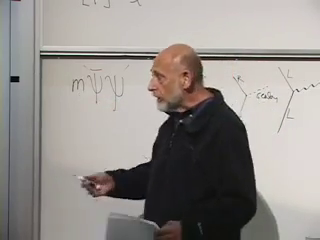
\includegraphics[width=0.76\textwidth]{lecture_01_figure_04.png}
\caption{Der Fermionmassenterm und die Skizzen der chiraliätsändernden Prozesse an der Tafel. Da ein Teil der Kreidezeichnungen verdeckt ist, werden die Diagramme im Folgenden algebraisch rekonstruiert.}
\lectureframe{01:23:36}
\end{figure}

In der gesprochenen Vorlesung ist oft von Händigkeit oder Helizität die Rede. Der genaue Schutz lässt sich am klarsten anhand der Chiralität formulieren. Für ein ultrarelativistisches Teilchen vermittelt das Helizitätsbild die gemeinte Anschauung; die von den links- und rechtshändigen Feldern in Gl.~\eqref{eq:fermion-mass} getragene Größe ist jedoch die Chiralität.

Eichwechselwirkungen erhalten die Chiralität:
\begin{equation}
L\xrightarrow{\ \gamma\ }L,
\qquad
R\xrightarrow{\ \gamma\ }R.
\label{eq:gauge-preserves-chirality}
\end{equation}
Eine Yukawa-Wechselwirkung mit einem Skalar koppelt entgegengesetzte Chiralitäten miteinander:
\begin{equation}
L\xleftrightarrow{\ \phi\ }R.
\label{eq:scalar-flips-chirality}
\end{equation}
Nehmen wir zunächst an, das Elektron habe anfangs \(m_0=0\). Die Emission und Reabsorption beliebig vieler Photonen kann keine Masse erzeugen, denn jeder Eichvertex erhält die Chiralität. Eine Folge von Wechselwirkungen, die links beginnt, bleibt links. Die reine Quantenelektrodynamik erlaubt somit konsistent ein masseloses Elektron: Seine elektromagnetische Selbstenergie kann keine additive Masse aus dem Wert null erzeugen.

Betrachtet man die Linien, beginnt man mit einem linkschiralen Elektron. Am ersten Photonvertex bleibt es linkschiral; nach der Ausbreitung und Reabsorption des Photons ist es ebenfalls noch linkschiral. Wiederholt man diese Konstruktion, fügt man lediglich weitere chiraliätserhaltende Vertizes ein. Die äußere Zweipunktfunktion kann renormiert werden, aber sie kann nicht die Links-rechts-Struktur annehmen, die eine Masse definiert.

Könnte eine Skalar-Emission das bewirken? Ein Skalarvertex wandelt \(L\) in \(R\) um, aber ein emittierter Skalar muss wieder absorbiert werden. Ein Zweipunkt-Selbstenergiediagramm enthält daher eine gerade Zahl von Skalarvertizes. Der zweite Flip kehrt den ersten um, sodass das vollständige Diagramm die äußere Chiralität erneut erhält. Ganz gleich, wie kompliziert das innere Diagramm wird: Emission und Reabsorption paaren die Vertizes miteinander und verhindern, dass bei verschwindender Anfangsmasse ein additiver Term von \(L\) nach \(R\) auftritt.

Das ist ein Paritätsargument bezüglich der Zahl der Flips. Ein Skalarvertex flippt die Chiralität einmal; damit jede innere Skalarlinie geschlossen wird, braucht es einen zweiten Endpunkt und damit einen zweiten Flip. Bei vier Skalarvertizes gibt es vier Flips und so weiter. Eine gerade Anzahl bringt das Fermion zu seiner ursprünglichen Chiralität zurück. Die Schlussfolgerung gilt nicht nur für die einfachste an der Tafel gezeichnete Schleife.

Eine von null verschiedene Massenkorrektur wird erst dann möglich, wenn das Diagramm bereits eine Masseneinsetzung enthält. Beispielsweise können Photonemission und -reabsorption eine Einsetzung von \(m_0\bar\psi\psi\) einschließen. Die Eichvertizes liefern zwei Potenzen der elektrischen Ladung, der einzige Chiralitätsflip hingegen die ursprüngliche Masse:
\begin{equation}
\begin{aligned}
m_e
&=m_0+c_1e^2m_0+c_2e^4m_0+\cdots\\
&=m_0\left(1+c_1e^2+c_2e^4+\cdots\right).
\end{aligned}
\label{eq:multiplicative-fermion-mass}
\end{equation}
Wenn \(m_0=0\) gilt, bleibt das Ergebnis null. Ist \(m_0\) klein, ist jede Korrektur proportional zu dieser kleinen Größe. Wir können weiterhin fragen, warum das Elektron im Vergleich zu einer fundamentalen Skala leicht ist, aber wir müssen nicht mehr große, voneinander unabhängige Zahlen voneinander abziehen, um diese Masse zu erhalten. In diesem Sinn ist eine kleine Fermionmasse technisch natürlich.

Die Masseneinsetzung macht die zulässige Abfolge deutlich. Man beginnt mit \(L\). Die Photonemission erhält \(L\); die Einsetzung \(m_0\) wandelt \(L\) in \(R\) um; die Reabsorption des Photons erhält \(R\). Das Diagramm hat nun die äußere Chiralität eines Massenterms, sein Wert enthält jedoch notwendigerweise den Faktor \(m_0\). Darin liegt der entscheidende Unterschied zu Gl.~\eqref{eq:one-loop-scalar-mass}, deren skalare Korrektur auch dann von null verschieden bleibt, wenn die anfängliche Skalarmasse auf null gesetzt wird.

Für Eichbosonen gibt es einen ähnlichen Schutz: Die Eichsymmetrie verbietet einen unabhängigen Massenterm, sodass ein masselos beginnendes Eichboson in allen Ordnungen der Störungstheorie masselos bleibt. Im Standardmodell entstehen die Massen der Fermionen und der schwachen Eichbosonen als Reaktion auf den Erwartungswert des Higgs-Feldes. Kontrolliert man die Higgs-Skala, erfordern die übrigen kleinen Massen keine eigenen Wiederholungen derselben katastrophalen Feinabstimmung.

Damit ist die Frage benannt, der sich die Supersymmetrie widmen soll: Kann eine Theorie verhindern, dass die Higgs-Skalargröße eine enorm große additive Massenkorrektur erhält? In passend supersymmetrischen Theorien lautet die Antwort ja, denn die bosonischen und fermionischen Beiträge sind miteinander verknüpft, statt unabhängig voneinander zu sein. Der genaue Mechanismus beginnt in der nächsten Vorlesung.

\section{Die andere Feinabstimmung: Vakuumenergie}

Es gibt ein noch schwerwiegenderes Renormierungsproblem, das jedoch erst beobachtbar wird, wenn die Gravitation einbezogen wird. In der nichtgravitativen Physik ändert eine additive Konstante, die zu jeder Energie hinzugefügt wird, kein Experiment. Die Elektronenmasse beispielsweise ist keine absolute Energie; sie ist die zusätzliche Energie, die nötig ist, um ein Elektron zum Vakuum hinzuzufügen:
\begin{equation}
m_e=E(\text{vacuum}+\text{one electron})-E(\text{vacuum})
\end{equation}
im Ruhesystem des Elektrons. Verschieben sich das Vakuum und jeder angeregte Zustand gemeinsam, bleiben ihre Energiedifferenzen unverändert.

Vakuum-zu-Vakuum-Diagramme verschieben dennoch die Vakuumenergie. In der Theorie \(\lambda\phi^4\) verbinde man die vier Beine eines quartischen Vertex zu zwei kurzen Schleifen. Jeder Propagator an einem Koinzidenzpunkt liefert \(1/\delta^2\), also gilt
\begin{equation}
\delta\rho_{\mathrm{vac}}
\sim
c_{\mathrm{vac}}\frac{\lambda}{\delta^4}.
\label{eq:vacuum-energy-divergence}
\end{equation}
Kompliziertere Vakuumdiagramme haben andere Kopplungsfaktoren und Koeffizienten, doch nach einer Dimensionsanalyse bleibt für eine Energiedichte typischerweise dieselbe quartische Cutoff-Abhängigkeit.

Gerade das Fehlen äußerer Linien kennzeichnet diese Korrektur. Zweipunktdiagramme vergleichen einen Einteilchenzustand mit dem Vakuum und verändern eine Masse; Vierpunktdiagramme verändern die Streuung; ein Diagramm ohne einlaufende oder auslaufende Teilchen verändert unmittelbar die Vakuum-zu-Vakuum-Amplitude. Ein quartischer Vertex liefert \(\lambda\), seine beiden kurzen Schleifen jeweils \(\delta^{-2}\). Nach einer Dimensionsanalyse folgt daraus die Energiedichteskala \(\delta^{-4}\).

Ohne Gravitation kann man den additiven Nullpunkt der Energie frei wählen und fragen, wen das kümmert. Die allgemeine Relativitätstheorie hebt diese Freiheit auf: Der Energie-Impuls-Tensor ist eine Quelle der Raumzeitkrümmung, sodass eine gleichförmige Vakuumenergie den leeren Raum gravitieren lässt. Sie tritt als kosmologische Konstante auf und steht in beobachtbarem Zusammenhang mit der dunklen Energie. Eine winzige gemessene Vakuumenergie muss dann Beiträge der Form \(\delta^{-4}\) überstehen.

Darum stellt sich die Frage anders, sobald die Gravitation eingeschaltet wird. In der gewöhnlichen Quantenmechanik lässt eine Verschiebung sämtlicher Energieniveaus um dieselbe Konstante alle Übergangsfrequenzen unverändert. In der Gravitation ist die Konstante nicht wirkungslos: Der Spannungstensor des Vakuums ist proportional zur Metrik und krümmt die Raumzeit. Was zuvor ein beliebig wählbarer Energie-Nullpunkt war, wird zu einer Quelle in Einsteins Gleichung.

Damit gibt es mindestens zwei extreme Natürlichkeitsprobleme. Die Vorlesung nennt für die Feinabstimmung der Vakuumenergie ungefähr 123 Dezimalstellen und für die Feinabstimmung der Higgsmasse ungefähr 30--35. Die genauen Zahlen hängen von der Ultraviolettskala und den Konventionen ab, doch der Unterschied steht außer Zweifel. Supersymmetrie könnte auf das hier besprochene Higgs-Problem antworten; wenn die Supersymmetrie gebrochen ist, erklärt sie für sich genommen jedoch nicht die beobachtete kosmologische Konstante.\editorialnote{Genau deshalb ist eine exakte Aufhebung zwischen Bosonen und --Fermionen keine phänomenologische Lösung für die beobachtete Vakuumenergie: In unserer Welt muss die Supersymmetrie gebrochen sein.}

\section{Abschließende Fragen aus dem Hörsaal}

\begin{classroomqa}
\audiencequestion{Die Higgs-Korrektur hängt vom Cutoff \(\delta\) ab, aber der Cutoff scheint beliebig gewählt. Könnte es die Planck-Länge, das Zehnfache der Planck-Länge oder etwas anderes sein? Wird dadurch die Feinabstimmung beliebig?\lecturetimestamp{01:33:50}}
\lecturerresponse{Der numerische Beitrag hängt von der kürzesten Skala ab, bis zu der man der effektiven Theorie vertraut. Diese Abhängigkeit ist Teil der physikalischen Buchführung und kein Ausweg. Moden bis hinunter zu jeder Skala, auf der das Standardmodell noch sinnvoll ist, sind Moden, deren Auswirkungen berücksichtigt werden müssen. Wählt man \(\delta\) als den Abstand, bei dem neue Physik erwartet wird---– vielleicht die Planck-Skala, vielleicht eine Vereinheitlichungsskala nahe \(10^{16}\,\mathrm{GeV}\) –, so ist der bis zu dieser Skala akkumulierte Beitrag bereits eine untere Schranke für das Problem. Führt man dieselbe Theorie zu noch kürzeren Abständen fort, wird die quadratische Abhängigkeit nur größer. Wir müssen erklären, wodurch der Beitrag von jeder Skala zwischen dem Labor und dieser ultravioletten Grenze aufgehoben wird.}
\end{classroomqa}

\begin{classroomqa}
\audiencequestion{Was kennzeichnet ein Skalarteilchen, und was ist ein Beispiel dafür?\lecturetimestamp{01:37:26}}
\lecturerresponse{Das Higgs ist das gemeinte Beispiel. Ein Skalar transformiert sich unter einer räumlichen Drehung nicht in verschiedene Komponenten; gleichbedeutend damit haben seine Teilchenquanten den Spin null. Das Photon wird durch ein Vektorfeld beschrieben, das Gravitationsfeld durch einen Tensor. Zum Zeitpunkt dieser Vorlesung im Jahr 2010 war noch kein elementares Teilchen mit Spin null nachgewiesen worden.\editorialnote{Das Higgs-Boson wurde am CERN im Jahr 2012 entdeckt; seine gemessenen Eigenschaften sind mit Spin null vereinbar.}}
\end{classroomqa}

\begin{classroomqa}
\audiencequestion{Ist das Teilchen \(Z\) ebenfalls ein Eichboson?\lecturetimestamp{01:38:31}}
\lecturerresponse{Ja. \(Z\), \(W^+\) und \(W^-\) sind Eichbosonen mit Spin eins, ebenso wie das Photon. Ihre Feldgleichungen und Wechselwirkungen sind nichtabelsche oder elektroschwache Verallgemeinerungen der eichfeldtheoretischen Beschreibung vom Maxwell-Typ.}
\end{classroomqa}

\begin{classroomqa}
\audiencequestion{Warum hebt der Beitrag des bosonischen Grundzustands den fermionischen Beitrag zur Vakuumenergie nicht auf?\lecturetimestamp{01:39:10}}
\lecturerresponse{Fermionenschleifen und die zugehörigen Bosonenschleifen können tatsächlich mit entgegengesetzten Vorzeichen eingehen. Eine Aufhebung erfolgt jedoch nicht automatisch: Teilchenmassen, Multiplizitäten und Kopplungen müssen übereinstimmen. Schon eine kleine Abweichung hinterlässt einen großen, vom Cutoff abhängigen Rest, und auch die unendlichen Familien von Diagrammen müssen sich Ordnung für Ordnung entsprechen. Exakte Supersymmetrie erzwingt genau solche Beziehungen zwischen Bosonen und --Fermionen. Eine allgemeine nichtsupersymmetrische Teilchenzusammensetzung tut das nicht; bei gebrochener Supersymmetrie bleibt ein Restproblem mit der Vakuumenergie bestehen.}
\end{classroomqa}

\section{Einordnung}

Der Aufbau der Vorlesung ist bewusst gewählt. Eine Molekülrechnung zeigt zunächst, dass das Eliminieren schneller Variablen weder einem Vernachlässigen noch einem Zaubertrick gleichkommt: Ihre Grundzustandsenergie wird zu einem Potential für die langsamen Variablen. Die Quantenfeldtheorie wiederholt diesen Vorgang über verschiedene Wellenlängen hinweg. Die Dimensionsanalyse zeigt anschließend, welche effektiven Parameter vom Cutoff abhängen. Skalarmassen erhalten additive Terme proportional zu \(\delta^{-2}\); eine kleine Higgs-Skala erscheint daher unnatürlich empfindlich. Fermionmassen werden multiplikativ renormiert, weil die Chiralität den Grenzfall verschwindender Masse schützt; die Eichsymmetrie schützt auf ähnliche Weise masselose Eichbosonen. Die Vakuumenergie reagiert noch empfindlicher und skaliert wie \(\delta^{-4}\); durch die Gravitation wird ihr absoluter Wert beobachtbar.

Die Supersymmetrie kommt genau an diesem Punkt im Kurs ins Spiel: nicht als schmückendes neues mathematisches Gerüst, sondern als Versuch, den Skalarsektor dem Verhalten der geschützten Sektoren ähnlicher zu machen. Als Nächstes gilt es zu verstehen, welche Symmetrie Bosonen und Fermionen so stark miteinander verknüpfen kann, dass ihre Aufhebungen geordnet ablaufen.